%!TEX root = presentazioneNBD.tex

\setlength{\parskip}{\baselineskip} 
\section{Applications}
\begin{frame}[t]
\begin{block}{Applications to Approximations Algorithms}
	\begin{itemize}
			\item Sparsest Cuts
            \item Flux, Expansion, and Minimum quotient separators
            \item Node cuts
			\item Minimum feedback arc set
            \item Geometric embeddings
        	\item Search Number
            \item Resistance, Conductance, and Rapidly-Mixing Markov Chains
	 \end{itemize} 
\end{block}
\end{frame}


%Networks
\begin{frame}
\frametitle{Introduction to applications}
Max-flow min-cut theorems can be applied to develop good approximation algorithms for a surprisingly wide variety of \textbf{NP-hard} problems. 

Graph partitioning is a critical component of many \textbf{"Dividi et Impera"} [\textit{Philip II of Macedon}] algorithms in practice. 

Unfortunately nearly every variation of the problem is NP-hard and little in the way of approximation algorithms has previously been discovered. 

\end{frame}


%Sparsest Cut
\begin{frame}[t]
\begin{block}{Applications to Approximations Algorithms}
	\begin{itemize}
			\item \textbf{Sparsest Cuts}
            \item Flux, Expansion, and Minimum quotient separators
            \item Node cuts
			\item Minimum feedback arc set
            \item Geometric embeddings
        	\item Search Number
            \item Resistance, Conductance, and Rapidly-Mixing Markov Chains
	 \end{itemize} 
\end{block}
\end{frame}

\begin{frame}
\frametitle{Sparsest Cut}
The sparsest cut of a graph $G=(V,E)$ is a partition $\left \langle U, \bar{U} \right \rangle$ for which:
$$\frac{\left | \left \langle U, \bar{U} \right \rangle \right |}{\left | U \right |\left | \bar{U} \right |}$$

is minimized, where $\left | \left \langle U, \bar{U} \right \rangle \right |$ denotes the number of edges connecting $U$ to $V-U$
\end{frame}

\begin{frame}
\centering
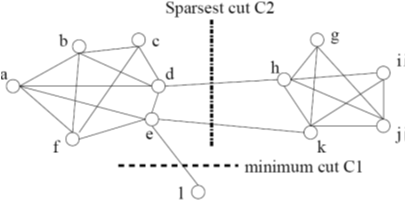
\includegraphics[width=\textwidth]{figs/sparsest_cut.png}
\end{frame}

\begin{frame}
Computing the sparsest cut of a graph is NP-hard .

The sparsest cut can be approximated to within an O(log n) factor using the SMALL CUT (UMFP) algorithm. 

In it's most general form, we desire to find  partition $\left \langle U, \bar{U} \right \rangle$ that minimize:

$$\frac{C(U,\bar{U})}{ \pi(U)\pi(\bar{U}) }$$

The sparsest cut can be approximated to within a factor of O(log p) using the PMFP methods. In this case, we set the capacity of an edge to equal its weight and $\pi(v)$ to be the node weight of v for all  V. 
\end{frame}

%FLUX

\begin{frame}[t]
\begin{block}{Applications to Approximations Algorithms}
	\begin{itemize}
			\item Sparsest Cuts
            \item \textbf{Flux, Expansion, and Minimum quotient separators}
            \item Node cuts
			\item Minimum feedback arc set
            \item Geometric embeddings
        	\item Search Number
            \item Resistance, Conductance, and Rapidly-Mixing Markov Chains
	 \end{itemize} 
\end{block}
\end{frame}

\begin{frame}
A graph has a flux at least $\alpha$if every subset U with at most half of the nodes is connected to the rest of the graph with edges of total weight at least a|U|. 
$$\alpha = \underset{U\subseteq V}{min} \frac{C( U, \bar{U})}{min(\left | U \right |,\left | \bar{U} \right |)} $$
A cut that achieves the flux is called the minimum quotient separator and is related by a constant factor to the sparsest cut since  
$$ \frac{n}{2} \mathscr{S} \le \alpha \le n \mathscr{S}$$
Computing the minimum quotient separator is NP-hard. The sparsest cut algorithms mentioned before provide O(log n).

\end{frame}


%Node Cuts

\begin{frame}[t]
\begin{block}{Applications to Approximations Algorithms}
	\begin{itemize}
			\item Sparsest Cuts
            \item Flux, Expansion, and Minimum quotient separators
            \item \textbf{Node cuts}
			\item Minimum feedback arc set
            \item Geometric embeddings
        	\item Search Number
            \item Resistance, Conductance, and Rapidly-Mixing Markov Chains
	 \end{itemize} 
\end{block}
\end{frame}

\begin{frame}
\frametitle{Node Cut}
Thus far, we have focused our attention on edge cuts for graphs.

These same methods can also be used to derive approximation algorithms for node cuts by converting the node-cut problem for an \textbf{undirected graph} into an edge-cut problem for a \textbf{directed graph}.

A node cut is a \textit{subset of nodes} whose removal from the graph separates the remaining nodes into two disconnected pieces.
\end{frame}

\begin{frame}

\centering
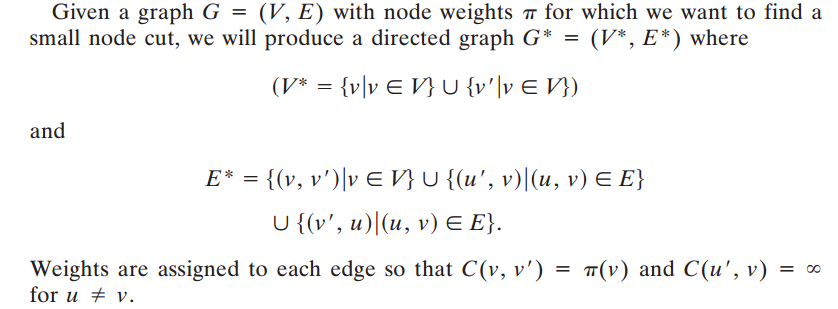
\includegraphics[width=\textwidth]{figs/node_cut.png}
\end{frame}

\begin{frame}
Any node cut in G corresponds to a directed edge cut in G* with the same cost and balance. 
 
The correspondence is as follows: Let U denote the set of nodes that cuts V - U into V1 and V2. 
 Then, the cut of $G^*$ is $\left \langle V^*_1, V^*_2 \right \rangle$  where $V^*_1=\left \{v|v \in V_1 \bigcup U\right \} \bigcup \left \{v'|v \in U \right \}$.
 
 And any directed edge cut in $G^*$ with noninfinite cost corresponds to a node cut in G with the same cost and balance. 
\end{frame}


%Minimum FeedBack arc set
\begin{frame}[t]
\begin{block}{Applications to Approximations Algorithms}
	\begin{itemize}
			\item Sparsest Cuts
            \item Flux, Expansion, and Minimum quotient separators
            \item Node cuts
			\item \textbf{Minimum feedback arc set}
            \item Geometric embeddings
        	\item Search Number
            \item Resistance, Conductance, and Rapidly-Mixing Markov Chains
	 \end{itemize} 
\end{block}
\end{frame}

\begin{frame}
\frametitle{Minimum FeedBack arc set}
The minimum feedback arc set problem
consists of removing the smallest number of edges F from a digraph G so that
the residual graph is \textbf{acyclic}. 

The problem is NP-hard and arises in numerous
applications.
An equivalent formulation of the problem is to find an ordering v1, v2, . . . , vn
of the nodes of G so that the number of forward edges F (i.e., edges of the form
(vi, vj) where i < j) is minimized. 
\end{frame}

\begin{frame}
In order to show that this algorithm produces an ordering with O(F log2n) forward edges where F is the optimal value for the graph, we again
examine the decomposition tree of subgraphs produced by the algorithm. In
particular, let $G_{i,j}$ denote the jth subgraph on level i of the decomposition tree,
and let $S_{i,j}$ denote the optimal directed bisection for $G_{i,j}$. 

Then the number of forward edges for the ordering produced by the algorithm is
\end{frame}

\begin{frame}
\centering
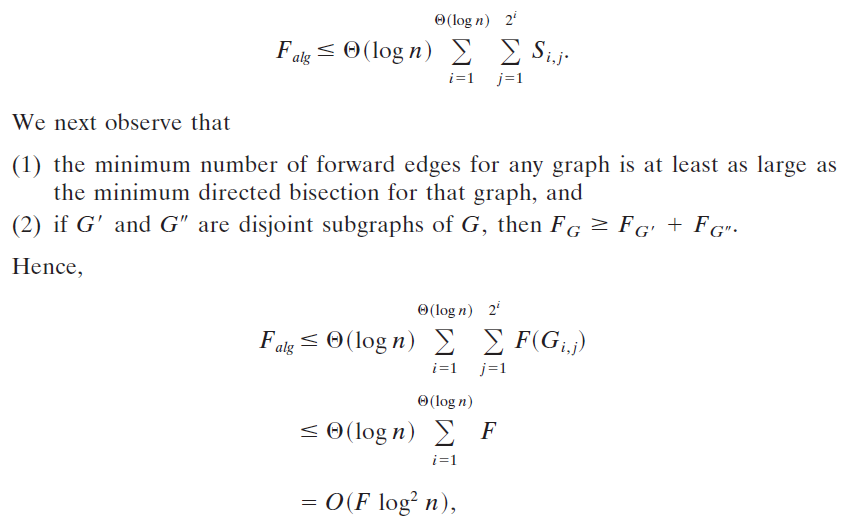
\includegraphics[width=\textwidth]{figs/Feedback_arc_set.png}
\end{frame}


%Geometric Embeddings
\begin{frame}[t]
\begin{block}{Applications to Approximations Algorithms}
	\begin{itemize}
			\item Sparsest Cuts
            \item Flux, Expansion, and Minimum quotient separators
            \item Node cuts
			\item Minimum feedback arc set
            \item \textbf{Geometric embeddings}
        	\item Search Number
            \item Resistance, Conductance, and Rapidly-Mixing Markov Chains
	 \end{itemize} 
\end{block}
\end{frame}


\begin{frame}
\frametitle{GEOMETRIC EMBEDDINGS}
The geometric embedding problem consists of
an edge-weighted graph $G=(V, E)$ and a set of points P in a d-dimensional
Euclidean space. 
The goal is to find an injection $f: V \rightarrow P$ that minimizes the
total edge length D induced on P, where
$$D =\sum_{
(u,v)\in E}
d(f(u), f(v))w(u,v)$$
d( x, y) is the Euclidean distance between points x and y, and w(u, v) is the
weight of edge (u, v). 
\end{frame}

\begin{frame}
From embedding into grids to embedding into an arbitrary graph H with small congestion and dilation. 
An embedding maps nodes of
G to nodes in H and edges in G to paths in H. 
\begin{itemize}
\item The congestion of the embedding
is the maximum for any edge e of H of the number of paths in the embedding
that contain e.
\item The dilation of an embedding is the maximum number of edges in
any path in the embedding.
\end{itemize}

THEOREM:
\textit{Consider any n-node bounded degree graph G and any 1–1
mapping h of the nodes of G onto the nodes of an n-node bounded degree graph H
with flux $\alpha$. The edges of G can be routed as paths in H with congestion and dilation
O(log n/$\alpha$).}

\end{frame}

%Search Number

\begin{frame}[t]
\begin{block}{Applications to Approximations Algorithms}
	\begin{itemize}
			\item Sparsest Cuts
            \item Flux, Expansion, and Minimum quotient separators
            \item Node cuts
			\item Minimum feedback arc set
            \item Geometric embeddings
        	\item \textbf{Search Number}
            \item Resistance, Conductance, and Rapidly-Mixing Markov Chains
	 \end{itemize} 
\end{block}
\end{frame}

\begin{frame}
\frametitle{ SEARCH NUMBER}
The search number of a graph is the number of searchers needed to capture a fugitive that can move with arbitrary speed about the edges of the graph.

A search step is the placing of
a searcher on a vertex, the movement along an edge, or the removal from a vertex. A search sequence is a sequence of search steps.

An edge e=( x, y) becomes clear when:
\begin{itemize}
\item there is a searcher on x and a second searcher moves from x to y
\item all the edges
other than e incident to x are clear and a searcher moves from x to y. 

A clear edge e can become contaminated again if the movement or removal of a searcher
results in a path from a contaminated edge to e that includes no nodes containing
a searcher.

\end{itemize}
\end{frame}

\begin{frame}
A search strategy for a graph is a search sequence that results in \textbf{
edges being simultaneously clear}. The search number of a graph is the minimum
number of searchers for which a search strategy exists.

Kirousis and Papadimitriou [1986] show that the node search number of a
graph is equal to its pathwidth plus one.  

Our results give an O(log2n)
approximation algorithm for finding the search number and node search number
of a graph.
\end{frame}


%RESISTANCE, CONDUCTANCE, AND RAPIDLY-MIXING MARKOV CHAINS.

\begin{frame}[t]
\begin{block}{Applications to Approximations Algorithms}
	\begin{itemize}
			\item Sparsest Cuts
            \item Flux, Expansion, and Minimum quotient separators
            \item Node cuts
			\item Minimum feedback arc set
            \item Geometric embeddings
        	\item Search Number
            \item \textbf{Resistance, Conductance, and Rapidly-Mixing Markov Chains}
	 \end{itemize} 
\end{block}
\end{frame}

\begin{frame}
\frametitle{RESISTANCE, CONDUCTANCE, AND RAPIDLY-MIXING MARKOV CHAINS.}

Reversible Markov Chains are often identified with a weighted directed graph
$G=(V, E)$ where the weight $\pi(v)$ of a node v is the probability of being in
state v in the stationary distribution and the weight $w(e)$ of an edge $e=(u, v)$ is
$\pi(u)P(u,v)$ where $P(u,v)$ is the probability of moving to state v from state u.
\begin{itemize}
\item The conductance C of the chain is equal to the flux of G and is useful in
quantifying the most severe transition bottleneck in the chain.
\item The resistance R of
the chain is the minimum capacity needed on each edge in order that there exist
a solution to the PMFP where $\pi(u)\pi(v)$ flow is passed between $u$ and $v$ $\forall
v \in V$. 
\end{itemize}
\end{frame}

\begin{frame} 
As a consequence of the inequality:
$$\Omega (\frac{\mathscr{S}}{log k}) \le f \le \mathscr{S}$$ , we can conclude that for any chain, $C^{-1}$ and
$R$ are equal up to a Q(log p) factor, where p is the number of non zero states in the chain.

A Markov chain is said to be rapidly-mixing if the chain reaches equilibrium
quickly. The mixing rate of a chain is often characterized in terms of its second
eigenvalue, which is known to be within a square of the conductance. 
\end{frame}

